\documentclass[border=10pt]{standalone}
\usepackage[svgnames]{xcolor}
\usepackage{amsmath}
\usepackage{pgfplots}
\pgfplotsset{compat=newest}
\usepackage[sfdefault]{FiraSans}
\usepackage{FiraMono}
\renewcommand*\familydefault{\sfdefault}
\begin{document}
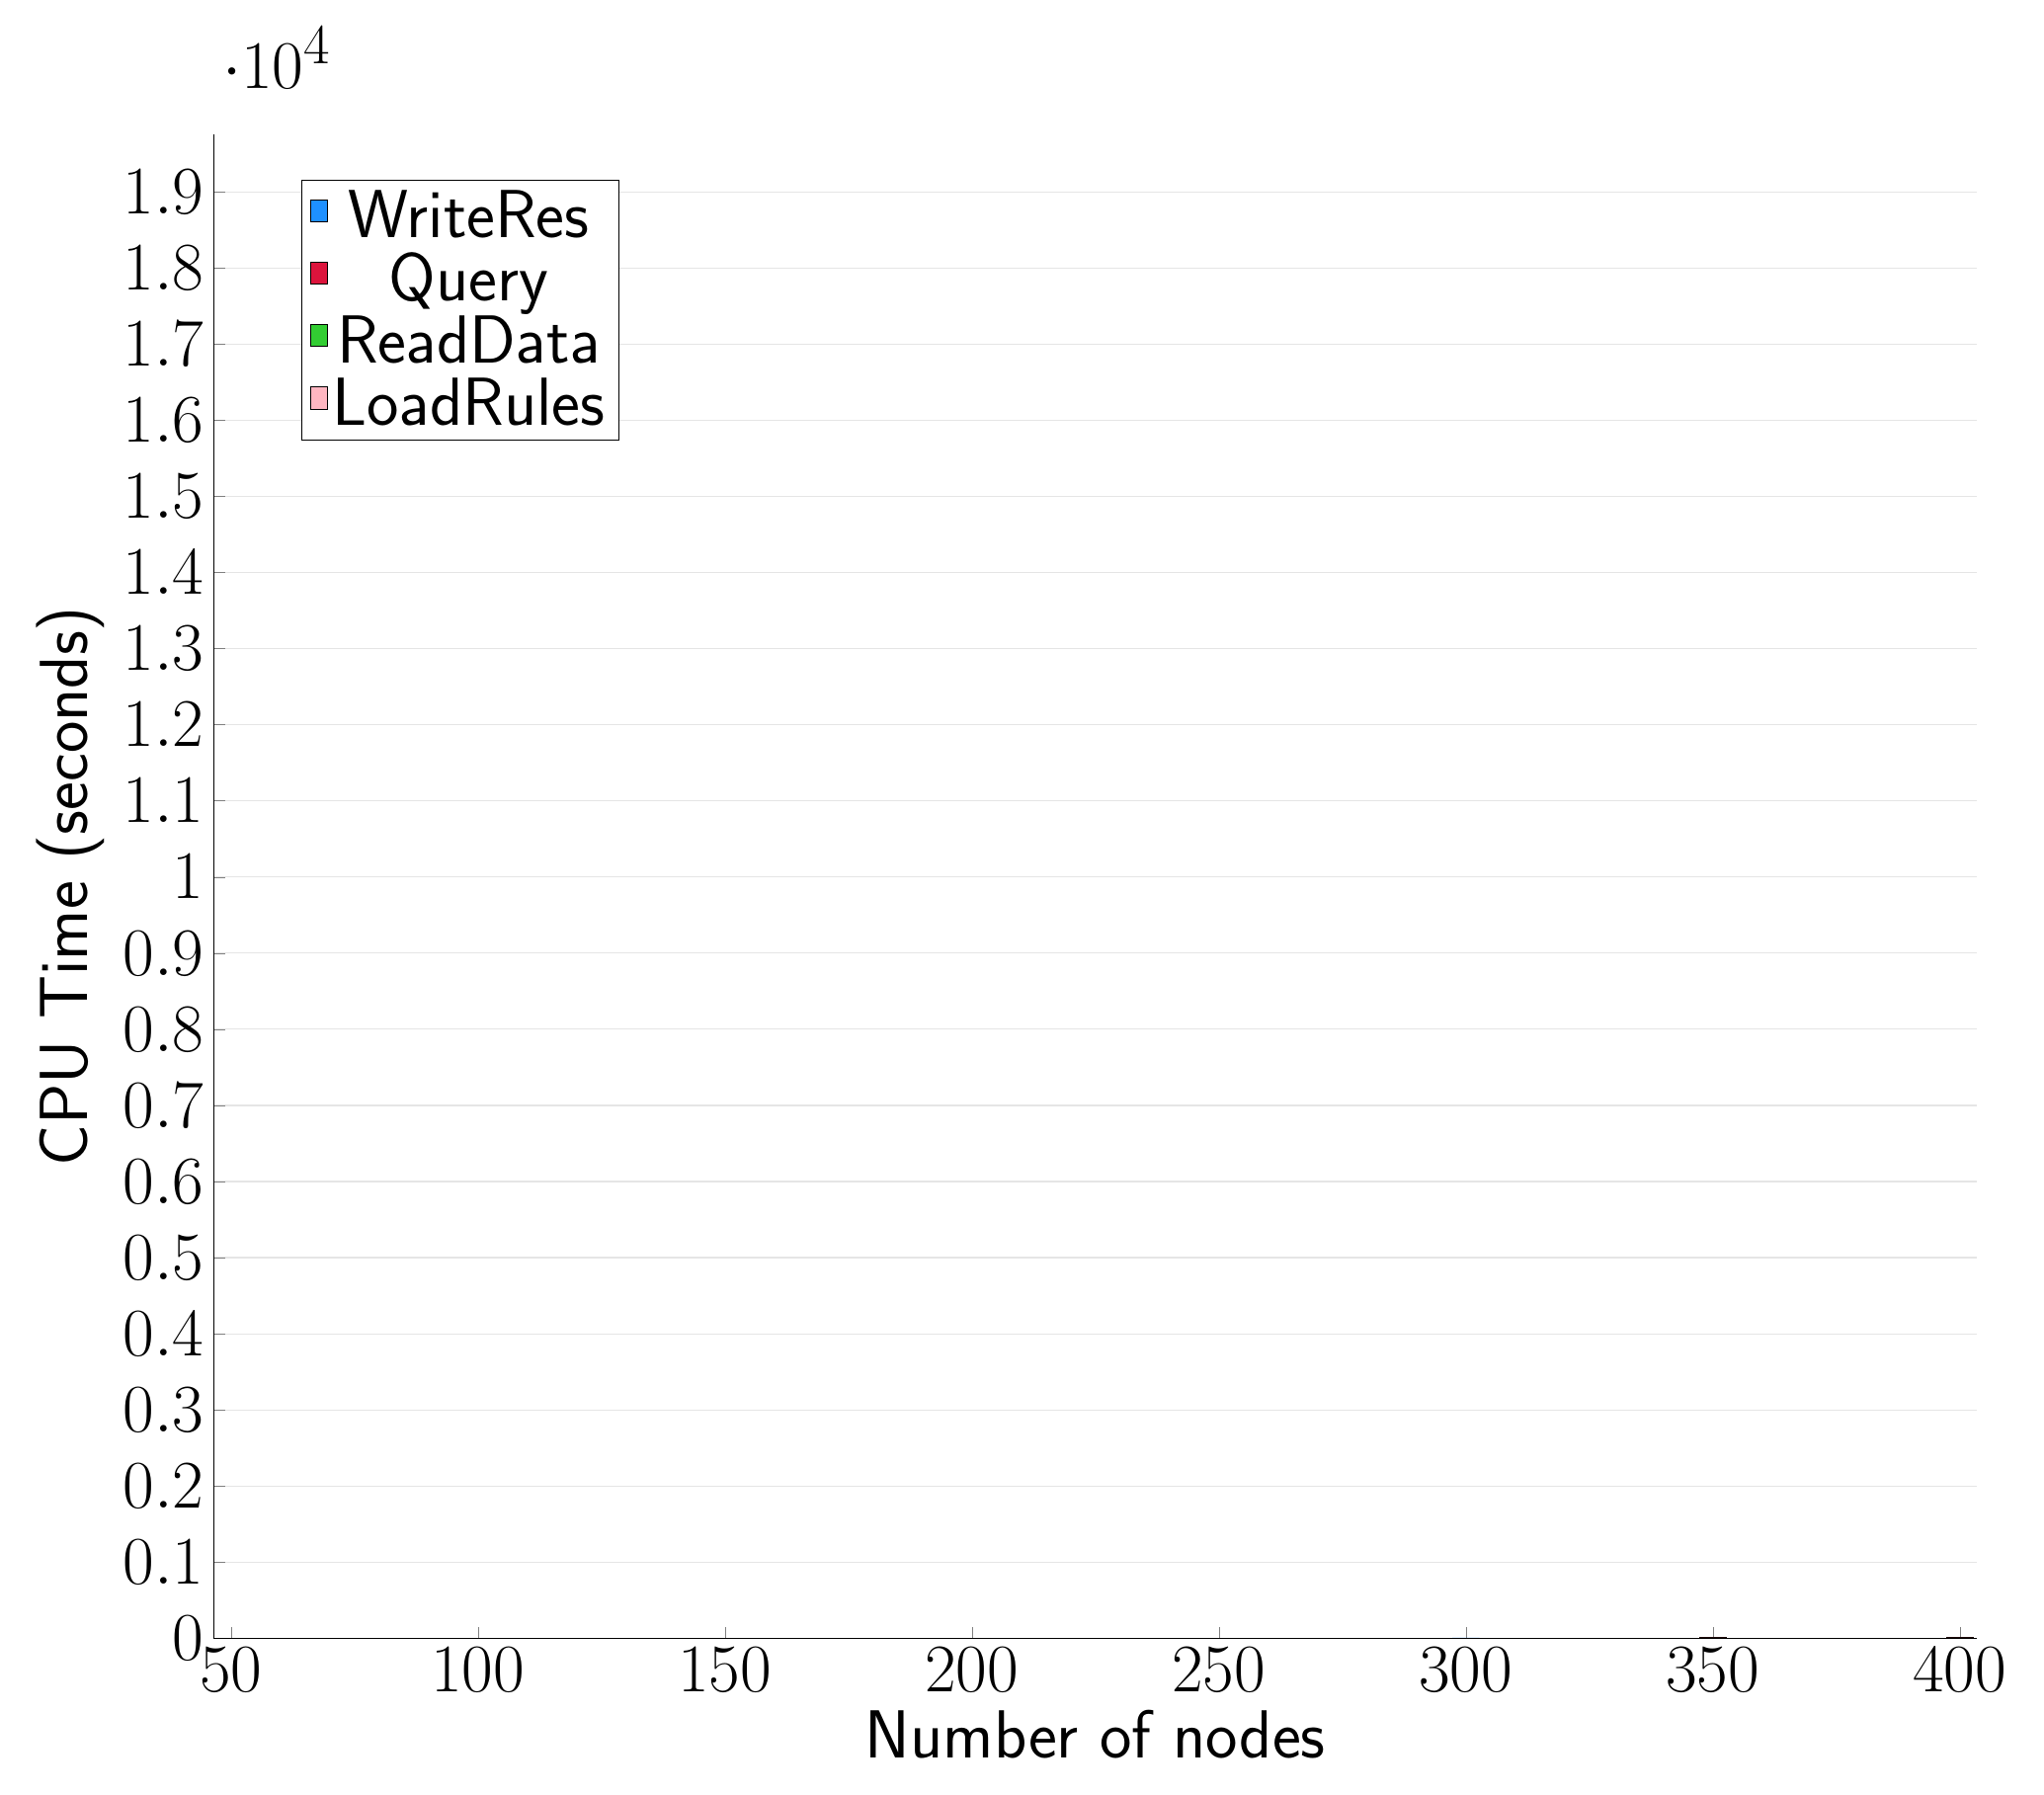
\begin{tikzpicture}
\begin{axis}[
   ybar stacked,
   width=2\textwidth,
   bar width=0.35cm,
   ymajorgrids, tick align=inside,
   major grid style={draw=gray!20},
   xtick=data,
   ymin=0, ymax=19758.773333333433,
   axis x line*=bottom,
   axis y line*=left,
   enlarge x limits=0.01,
   legend style={
       at={(0.23, 0.97)},
       anchor=north east,
       legend columns=1,
       font=\Huge,
   },
   ylabel={CPU Time (seconds)},
   xlabel={Number of nodes},
   label style={font=\Huge},
   tick label style={font=\Huge},
]
\addlegendimage{fill=DodgerBlue, draw=black, line width=0.2pt}
\addlegendentry{WriteRes}
\addlegendimage{fill=Crimson, draw=black, line width=0.2pt}
\addlegendentry{Query}
\addlegendimage{fill=LimeGreen, draw=black, line width=0.2pt}
\addlegendentry{ReadData}
\addlegendimage{fill=LightPink, draw=black, line width=0.2pt}
\addlegendentry{LoadRules}
\addplot +[fill=LightPink, draw=black, line width=0.2pt] coordinates {
(50, 0.003363)
(100, 0.004844333333333333)
(150, 0.004873333333333333)
(200, 0.0024813333333333332)
(250, 0.0028606666666666663)
(300, 0.0033216666666666668)
(350, 0.0028299999999999996)
(400, 0.0022903333333333335)
};
\addplot +[fill=LimeGreen, draw=black, line width=0.2pt] coordinates {
(50, 0.022923666666666665)
(100, 0.13818866666666665)
(150, 0.22122799999999998)
(200, 0.38070266666666663)
(250, 0.5642263333333334)
(300, 0.9096676666666667)
(350, 1.3678083333333335)
(400, 1.6544413333333334)
};
\addplot +[fill=Crimson, draw=black, line width=0.2pt] coordinates {
(50, 0.007850333333333334)
(100, 0.085877)
(150, 0.19569499999999998)
(200, 0.46140566666666666)
(250, 0.9926756666666666)
(300, 1.6475333333333333)
(350, 2.795145)
(400, 4.230827000000001)
};
\addplot +[fill=DodgerBlue, draw=black, line width=0.2pt] coordinates {
(50, 0.08429766666666667)
(100, 0.43644066666666664)
(150, 0.6691196666666667)
(200, 1.1822226666666666)
(250, 1.7963913333333335)
(300, 2.571315333333333)
(350, 3.364259)
(400, 4.795075000000001)
};
\end{axis}
\end{tikzpicture}

\end{document}
